\subsection{Introduction to Naiads software interface}
\noindent This is the interface to understand the current communication of the system to help analyse and add new programs. If something is unclear the best way is to check the code for that program/node.\\ Reservation for small mistakes such as spelling of fields in JSON object etc. The field names can also be confirmed in the code.\\
All code should be commented and written with a standard such as:
\begin{description}
  \item[variables] starts with lower-case letter, other words with Upper-case as first letter. Each variable should start with what type it is (example unsigned_16 : u16VariableName). The name should be descriptive of its purpose.
  \\if special type the type name is x (example special type : xVariableName).
  \item[functions/procedures] Should start with upper-case letters in each word and each word separated with underline (example This_Is_A_Procedure).
  \item[Libraries/files] Should follow same standard as functions/procedures.
  \item[Comments] All procedures and functions shall have comments on their purpose and as much as possible on why and how.
\end{description}

\subsection{BeagleBone Black}
\noindent For creating a new node you need to use the library TCP_Client's function Set_IP_And_Port at IP 192.168.1.1 with a 3 letter long name written in lower-case, which will be transferred to a unique port number.
All communication intern this system will be with JSON objects with all fields in lower case letters.
Following nodes is currently implemented and with the interface toward each of them, the first 3 letters is the target name.


\begin{figure}[!ht]
	\begin{center}
		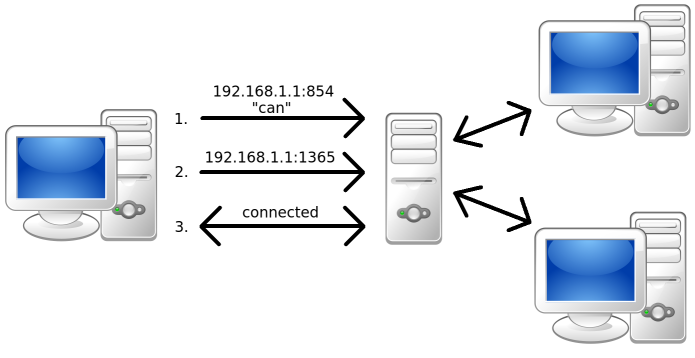
\includegraphics[width=80mm]{./Images/Software/tcp_init_connection.png}
		\caption{Initial TCP communication messages}
		\label{YourLabel}
	\end{center}
\end{figure}


\newline \noindent If the library TCP_Client is not used, the initial set-up and communication software has to be implemented again. As clients are only supposed to be connected to the server node, they only need one connection. To make a successful connection the client should first connect to port 854. This connection is just to send a short message to the server, telling the name of the client. The name is a three character long string. It should be the same three characters as what other clients are using when they want to send a message to the this client. When the message is sent, the server will open a new server connection on a port that is based on the clients name. This is the connection where the client can now connect and where it can communicate with other clients. There will be a short delay before the server have successfully configured the new connection so if the client is trying to connect too soon after the initial message, it will fail and the client will have to retry. The port number is calculated by using the each letters as a number in base 26. It makes the possible port range go from 0 (aaa) to 17576 (zzz). A list of current name and the corresponding ports can see in “port.txt”. All messages sent should always at least contain the two variables target and a sender. The variable target is a three character long string that should correspond to the name of the node which should receive the message and sender similar but it should instead be the name of the client that is sending the message. Another useful variable tag that is used are ethid, which tells the receiver what type of message it is. Another important thing the client has to consider is that all message should always be exactly 256 bytes. This is because the server will only react when its buffer is full, which is when it receives 256 bytes on a connection. The safest way to fill a message is by padding the message with spaces (ASCII value 32). When a client is waiting to receive a message, it should also expect a message size of 256 bytes. The server will never drop the connection intentionally. If the connection is broken, it will be because an issue with the server, like a crash or it can mean that the physical connection is broken. 



\newline \noindent All of the procedures above can be handled by a client library called “tcp_client” that is written in ADA. This library will only be able to handle one connection and it is done by a separate thread that is running as soon as the library is included. As soon as the initialization procedure is called, it will connect properly and allow the client to send and receive messages from anywhere in the program. This will also pad messages automatically and it will clean up received messages. The thread that handles the connection will also automatically try to reconnect to the server if the connection is lost.





\subsubsection{bgw - boarder gate way}
The main node routing all messages, all programs will connect to this one. User("usr") and simulation("sim") have the possibility to tell this node that it wants to listen to desired messages
\begin{description}
  \item["target"] (string) name of the target with 3 letters (a-z).
  \item["ehtid"] (integer) which setting to change where 2 is to mirror data and 3 is to block data flow
  \item["xxx"] (boolean) true or false, xxx is the name of the node that the setting should effect.
\end{description}

\subsubsection{usr - user}
A computer connected to Naiad, may listen to messages to simulate in real-time, or send missions to the mission control node etc.
\begin{description}
  \item["target"] (string) "usr"
  \item["sender"] (string) "pid".
\end{description}




\subsubsection{sns - sensor}
Handles all sensor data, sensor fusion and sending the data to the nodes that needs it.
will get following message for update position and orientation
\begin{description}
  \item["target"] (string) "sns"
  \item["sender"] (string) "can".
  \item["accx"] (float) accelerometer x.
  \item["accy"] (float) accelerometer y.
  \item["accz"] (float) accelerometer z.
  \item["roll"] (float) roll angle (in degrees).
  \item["pitch"] (float) pitch angle (in degrees).
  \item["yaw"] (float) z angle (in degrees).
\end{description}

\subsubsection{pid - PID-controller}
Calculates the needed values of the thruster to get to desired position and orientation.
Can be absolute or relative coordinate/orientation.
Message to set this is structured as following:
\begin{description}
  \item["target"] (string) "pid".
  \item["sender"] (string) name of sender, most often "pth".
  \item["ethid"] (integer) 1 if absolute coordinate, 2 if relative.
  \item["posx"] (float) x coordinate (in meters).
  \item["posy"] (float) y coordinate (in meters).
  \item["posz"] (float) z coordinate (in meters).
  \item["roll"] (float) roll angle (in degrees).
  \item["pitch"] (float) pitch angle (in degrees).
  \item["yaw"] (float) z angle (in degrees).
\end{description}
Sends following after thruster values been calculated:
\begin{description}
  \item["target"] (string) "can".
  \item["sender"] (string) "pid".
  \item["ethid"] (integer) 616 (can identifier for thruster values).
  \item["len"] (integer) 6.
  \item["b1".."b6"] (integer(value 0 to 255)) value for thruster n.
\end{description}

\subsubsection{pth - Path-planner}
Gets positions and orientation from mission control and updates the PID-controllers desired values to get there.
Updates the PID when new sensor data or new desired positions comes. 
\begin{description}
  \item["target"] name of the target with 3 letters (a-z).
  \item["sender"] name of the node sending  with 3 letter (a-z).
\end{description}

\subsubsection{msn - mission-control}
Getting feedback from cameras and sensor to help complete missions by telling the path planner where to go.
\begin{description}
  \item["target"] name of the target with 3 letters (a-z).
  \item["sender"] name of the node sending  with 3 letter (a-z).
\end{description}

\subsubsection{can - CAN-translator}
Sends the CAN-messages to the correct program on BBB, and sends messages from BBB to the CAN-bus.\\
When a JSON message with the field target as "can", this node will receive that message and send it to the CAN-bus with following settings.
\begin{description}
  \item["target"] (string) can
  \item[ethid] (integer) can identifier (0-2047)
  \item["len"] (integer) number of bytes in message (1-8)
  \item["b0".."bn".."b7"] (integer) byte data 0-255, in index n
\end{description}

\subsubsection{vsf - vision front}
Will send distance, hight difference and yaw angle to the object of interest.
The format of one of those messages is:
\begin{description}
  \item["target"] (string) "msn".
  \item["sender"] (string) "vsf".
  \item["yaw"] (float) yaw value to object.
  \item["x"] (float) distance in horizontal to object.
  \item["z"] (float) distance in vertical to object.
\end{description}

\subsection{CAN cards}
\noindent 
To program the CAN-cards in Ada one will need to download and install GNAT Ada GPL 2012 for AVR microcontroller ELF format (windows).\cite{link to download}  to compile Ada code for the AT90CAN128. To download the code to the microcontroller use Atmel Studio\cite{Atmel Studio}.
\\The AT90CAN128 should have the following configurations: \\
\\
BODLEVEL = DISABLED\\
TA0SEL = [ ]\\
OCDEN = [ ]\\
JTAGEN = [X]\\
SPIEN = [X]\\
WDTON = [ ]\\
EESAVE = [ ]\\
BOOTSZ = 4096W_F000\\
BOOTRST = [ ]\\
CKDIV8 = [ ]\\
CKOUT = [ ]\\
SUT_CKSEL = EXTXOSC_8MHZ_XX_16KCK_0MS\\
\\
EXTENDED = 0xFF (valid)\\
HIGH = 0x99 (valid)\\
LOW = 0xDF (valid)\\
\\
\\
The tool used to download the code to the microcontoller was JTAGICE3\cite{JTAGICE3} and JTAGICE MKII\cite{JTAGICEMKII} 

To connect a new node simply connect a new node that communicate at a baud rate of 250000 bits/second. Following nodes are currently connected to the CAN-Bus and will have one section for outgoing message(if any) and for what messages they listen to(if any).

\subsubsection{Ask for name of all nodes}
If a message with Identifier 380 is sent, all nodes (except PSU) will return there name to PSU node. This can be used to check that all nodes are still alive.

\subsubsection{Example message}
\begin{description}
  \item[ID] Identifier number and if extended or not, for example (580, false), so far extended is never used.
  \item[Len] Number of Bytes of data to be sent.
  \item[Data] as array with position 1 to 8 values 0-255.
\end{description}

\subsubsection{Thruster}
If no messages received in last 1.0 seconds motors is set to neutral to avoid movement if something goes wrong in higher levels.
Incoming messages:
\begin{description}
  \item[616] 6 bytes of data, data(1) speed of motor 1, .. , data(6) speed of motor 6.
  \item[623] 1 byte, value 0-100, sets a software limit for the motor, value in percent, recommended to not go above 50%.
\end{description}


\subsubsection{Sensor}
Current for pressure/depth sensor, shield is able to connect to salinity and temperature also.\newline
outgoing messages:
\begin{description}
  \item[1593] 2 bytes from pressure sensor, updated at 10 Hz.
\end{description}


\subsubsection{INS}
This card will send values from the inertial measurement unit and fiber optic gyro(when done), as 32 bits float values.\newline
update frequency 20 Hz.\newline
outgoing messages:
\begin{description}
  \item[1594] byte 1-4 : Yaw, byte 5-8 : Pitch.
  \item[1595] byte 1-4 : Roll, byte 5-8 : Accelerometer Z.
  \item[1596] byte 1-4 : Accelerometer X, byte 5-8 : Accelerometer Y.
\end{description}



\subsubsection{Power supply unit}
The node activating all others electronics (BBB, can-bus etc).
Following is done at startup: \newline
Starting electronics, sets port A, bit 4 to true. \newline
Starting motors, sets port A, bit 3 to true. \newline
Incoming messages:\newline
\begin{description}
  \item[480] Restart system
  \item[481] Turn off system
  \item[482] Turn on system
  \item[486] allow auto self restart
  \item[487] don't allow auto self restart
  \item[489] Clear LCD
  \item[490-497] write text on LCD, 
  \item[501] Requests a list of connected CAN-cards 
  \item[504] ping message to tell PSU that the rest of the system is running
  \item[510] print Naiad on LCD
\end{description}
outgoing messages:
\begin{description}
  \item[400] Stop mission (if mission switch gets attached) %check theese two might be switched
  \item[404] Start mission (if mission switch gets removed)
  \item[1000] Name of a connected node byte 1-8 in ascii value filled out with spaces after name.
\end{description}



\subsubsection{LED}
Control the LED strips on the wings.
incoming messages:
\begin{description}
  \item[753] Turn of all lights
  \item[754] turn on port/starboard blinking
  \item[755] turn of port/starboard blinking
  \item[756] set left wing, if byte 1-6 /= 0 set led(1-6) = true
  \item[757] set right wing, if byte 1-6 /= 0 set led(1-6) = true
  \item[760] set pwm (data(1)) for front spotlight, value 0-255
  \item[761] set pwm (data(1)) for bot spotlight, value 0-255
\end{description}

\subsubsection{Solenoid}
Controlling up to 4 solenoids, by opening for 2.5 seconds then closing them.
incoming messages:
\begin{description}
  \item[988] activate port 0.
  \item[989] activate port 1.
  \item[990] activate port 2.
  \item[991] activate port 3.
\end{description}




\subsubsection{Example node}



